% Defense slides — 12 min, Politecnico di Torino
% Build: latexmk -pdf slides.tex  (figures pulled from ../)
\documentclass[aspectratio=169,10pt]{beamer}
\usetheme[progressbar=frametitle]{metropolis}
\usepackage{amsmath,amssymb}
\usepackage{graphicx}
\graphicspath{{../assets/figures/}}
\usepackage[style=authoryear,maxcitenames=1]{biblatex}
\addbibresource{../bib.bib}

\setbeamertemplate{frame numbering}[fraction]
\setbeamerfont{footnote}{size=\tiny}

\title{Can a simple model explain economics?}
\subtitle{Firm-growth statistics from disordered Lotka--Volterra dynamics}
\author{Ludovico Furlanetto}
\date{July 2026}

\begin{document}

% title page laid out like the thesis titlepage: Candidate / Supervisors side by side
\begin{frame}[plain]
  \vspace*{2mm}
  \noindent{\small Master's Degree in Physics of Complex Systems}%
  \hfill\raisebox{-3mm}{
\includegraphics[height=1cm]{polito_logo.png}}

  \vfill
  {\usebeamercolor[fg]{title}\LARGE\bfseries Can a simple model explain economics?\par}
  \vspace{2mm}
  {\color{gray}\rule{\textwidth}{0.4pt}}\par
  \vspace{2mm}
  {\large Firm-growth statistics from disordered Lotka--Volterra dynamics\par}
  \vfill
  \begin{minipage}[t]{0.46\textwidth}
    \raggedright
    {\small\bfseries Candidate}\par\vspace{1.5mm}
    Ludovico Furlanetto
  \end{minipage}\hfill
  \begin{minipage}[t]{0.46\textwidth}
    \raggedleft
    {\small\bfseries Supervisors}\par\vspace{1.5mm}
    Fabi\'an Aguirre-L\'opez\\
    Luca Dall'Asta
  \end{minipage}
  \vfill
  \centering July 2026
  \vspace*{2mm}
\end{frame}

% ---------------------------------------------------------------- 1 min
\begin{frame}{Two robust facts about firm growth}
  Annual log-growth rates $g_i = \Delta \log S_i$, conditioned on firm size $S$:
  \begin{enumerate}
    \item \alert{Size--variance relation}: volatility falls slowly with size,
      \[ \sigma(S) \sim S^{-\beta}, \qquad \beta \approx 0.15\text{--}0.20 \]
      far from the $\beta = 1/2$ of independent sub-units.
    \item \alert{Fat-tailed growth rates}: the distribution of $g$ is
      tent-shaped, not Gaussian, with heavy tails that \emph{strengthen} with firm size.
  \end{enumerate}
  \medskip
  Both hold across countries, decades, and definitions of size.
\end{frame}

\begin{frame}{The granular explanation, and where it fails}
  \textbf{Standard picture}: a firm is a collection of independently fluctuating
  sub-units (plants, products) with heavy-tailed sizes. Both facts then follow from
  internal composition.
  \medskip

  \textbf{Moran et al.\ (2024)}: condition the higher moments on size,
  $\langle |g|^q \,|\, S\rangle \sim S^{-\zeta_q}$. The data multiscale:
  \[ \zeta_q/\zeta_1 \;=\; 1,\; 2.0,\; 2.6,\; 2.9 \qquad (q = 1,\dots,4) \]
  \begin{itemize}
    \item granular models predict a \emph{flat} ratio curve beyond $q=1$,
    \item a size-dependent volatility with fixed shape predicts the straight line $\zeta_q/\zeta_1 = q$,
    \item the data lie between --- neither works.
  \end{itemize}
  Their suggestion: shocks to a firm's sub-units must grow \emph{more correlated} with its size.
\end{frame}

\begin{frame}{The question}
  \begin{center}
    {\Large Can a dynamical model of \alert{interacting firms} generate both facts on its own?}
  \end{center}
  \bigskip
  \begin{itemize}
    \item no internal sub-unit structure,
    \item no external noise --- fluctuations generated by the interactions themselves,
    \item statistics measured exactly as in the empirical work.
  \end{itemize}
\end{frame}

% ---------------------------------------------------------------- 3 min
\begin{frame}{The model: relative Lotka--Volterra on a scale-free graph}
  Generalized Lotka--Volterra, made scale-invariant by measuring every firm
  against the average firm $m$:
  \[
    \dot{x}_i = x_i \left( 1 - \frac{x_i}{m} + \frac{(Wx)_i}{m} \right)
    + \lambda\,(m - x_i),
    \qquad m = \frac{1}{N}\sum_j x_j
  \]
  \begin{itemize}
    \item $W_{ij} = A_{ij}\left(\frac{\mu}{C} + \frac{\sigma}{\sqrt{C}} z_{ij}\right)$:
      quenched Gaussian couplings on a configuration-model graph with power-law
      degrees (tail exponent $2.5$, mean degree $C = N/40$),
    \item invariant under $x \to c\,x$: no preferred size, competition acts on
      \emph{market share} $x_j/m$,
    \item $\lambda = 10^{-3}$: entry flow of small firms, prevents exact extinction.
  \end{itemize}
  \medskip
  In relative sizes $S_i = x_i/m$ this is a replicator equation: firms gain share
  when their fitness beats the market average.
\end{frame}

\begin{frame}{Phases: where the economy keeps fluctuating}
  \begin{columns}
    \column{0.55\textwidth}
      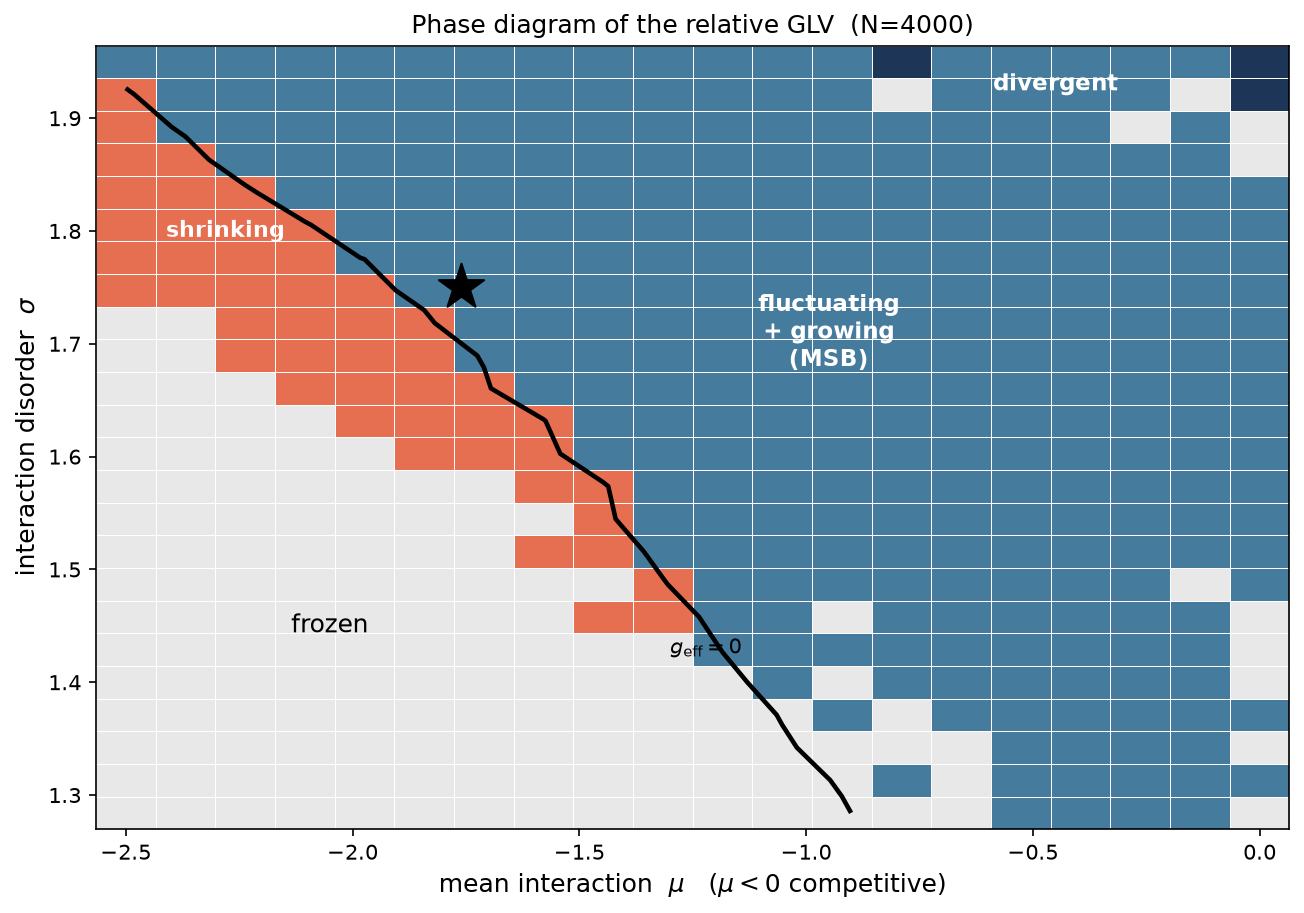
\includegraphics[width=\textwidth]{phase_diagram.png}
    \column{0.42\textwidth}
      \begin{itemize}
        \item weak disorder: composition freezes at a fixed point --- growth rates vanish,
        \item strong disorder: the replicator flow stays \alert{chaotic}; the scale $m$
          grows exponentially while the composition churns forever,
        \item operating point $\mu = -1.76$, $\sigma = 1.75$: competitive,
          deep in the fluctuating phase.
      \end{itemize}
      \medskip
      All statistics are \emph{stationary} properties of this state.
  \end{columns}
\end{frame}

% ---------------------------------------------------------------- 5 min
\begin{frame}{Both facts emerge in the fluctuating state}
  \begin{center}
    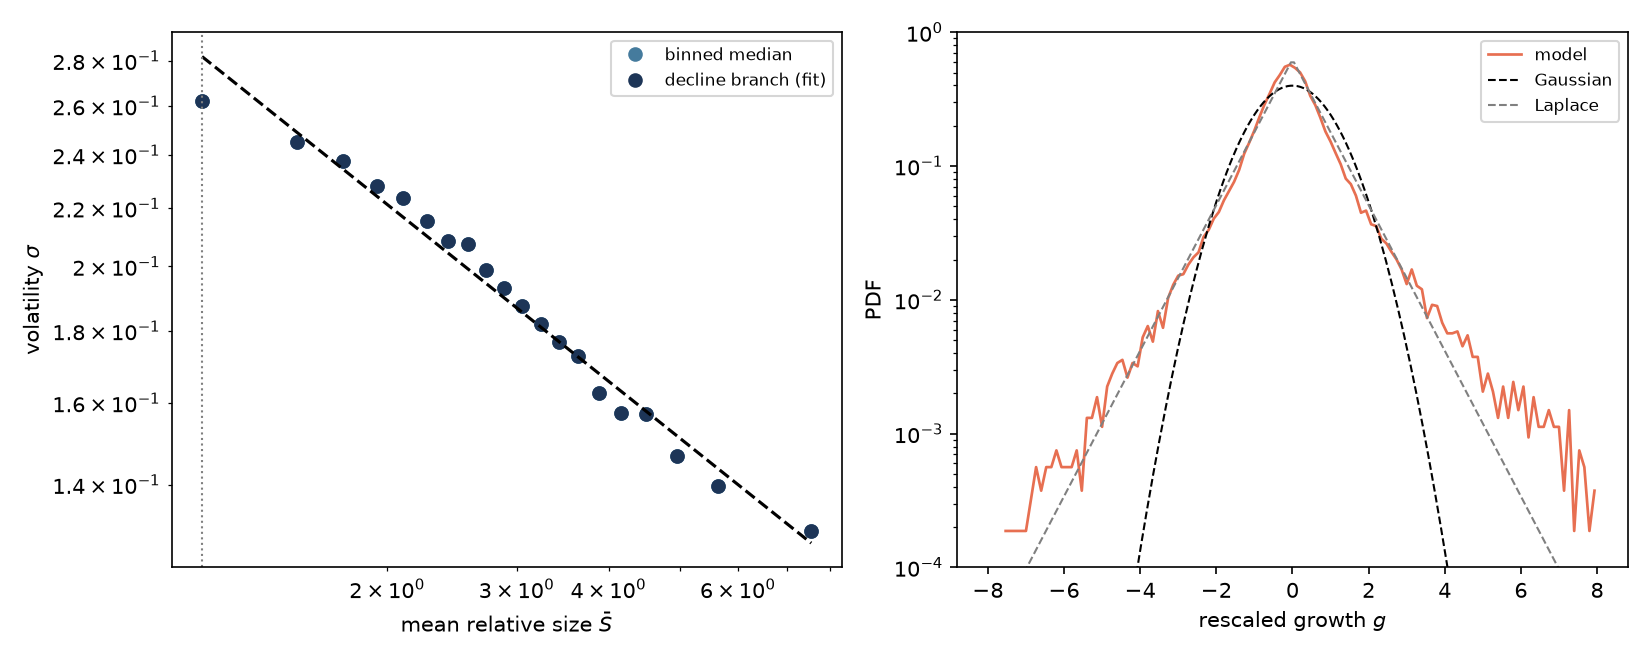
\includegraphics[height=0.58\textheight]{meandeg_stationary_msb.png}
  \end{center}
  \begin{itemize}
    \item \textbf{Left}: clean size--variance power law, $\beta = 0.45 \pm 0.06$
      per economy, $R^2 = 0.99$ ($N = 16000$, twenty economies),
    \item \textbf{Right}: tent-shaped, fat-tailed growth-rate distribution --- no external noise put in.
  \end{itemize}
\end{frame}

\begin{frame}{The multiscaling test}
  \begin{center}
    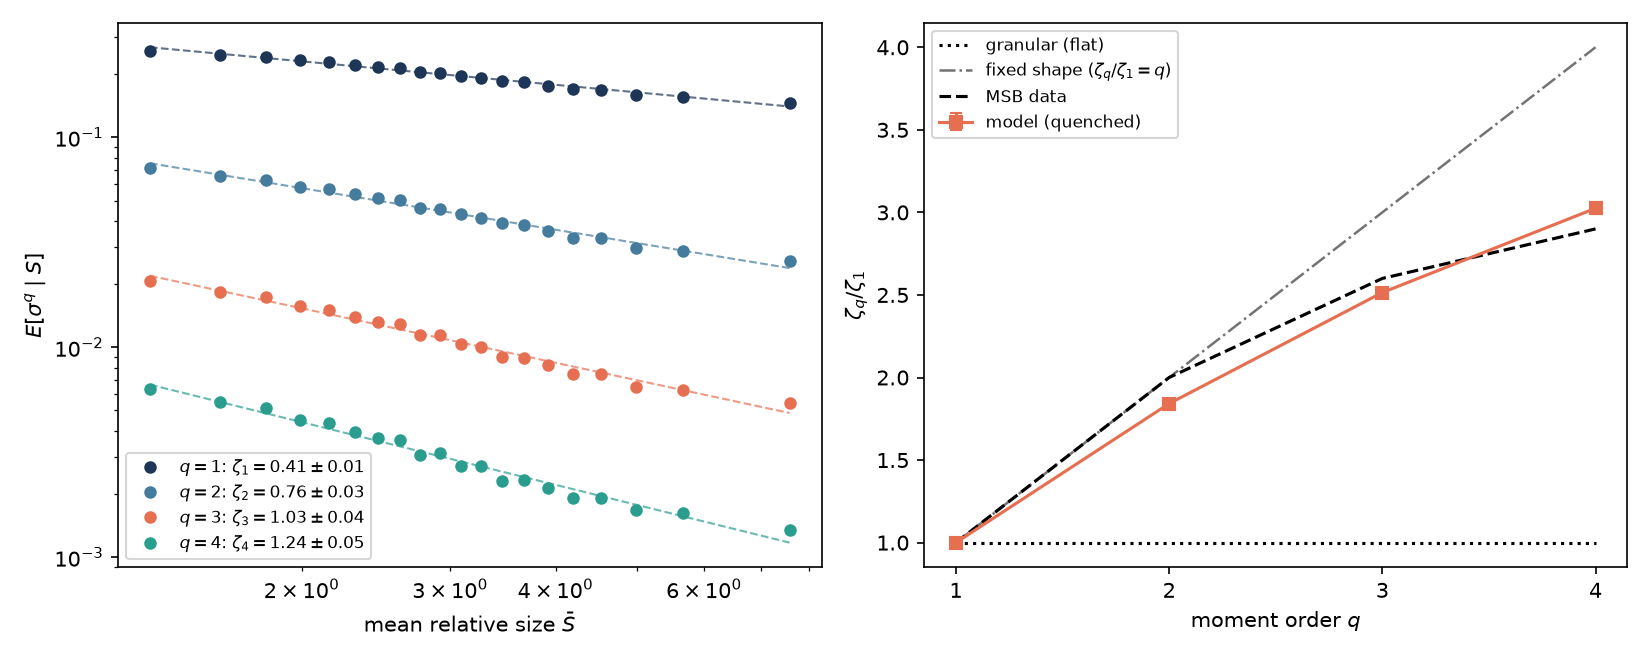
\includegraphics[height=0.55\textheight]{meandeg_multiscaling.png}
  \end{center}
  \begin{itemize}
    \item higher-moment exponents $\zeta_1,\dots,\zeta_4 = 0.41,\, 0.76,\, 1.03,\, 1.24$,
    \item normalized: $\zeta_q/\zeta_1 = 1,\; 1.84,\; 2.51,\; 3.02$
      vs.\ empirical $1,\; 2.0,\; 2.6,\; 2.9$,
    \item bent below the fixed-shape line $\zeta_q/\zeta_1 = q$ by many standard errors ---
      the anomalous multiscaling that ruled out the granular picture.
  \end{itemize}
\end{frame}

\begin{frame}{The graph is the mechanism}
  \begin{center}
    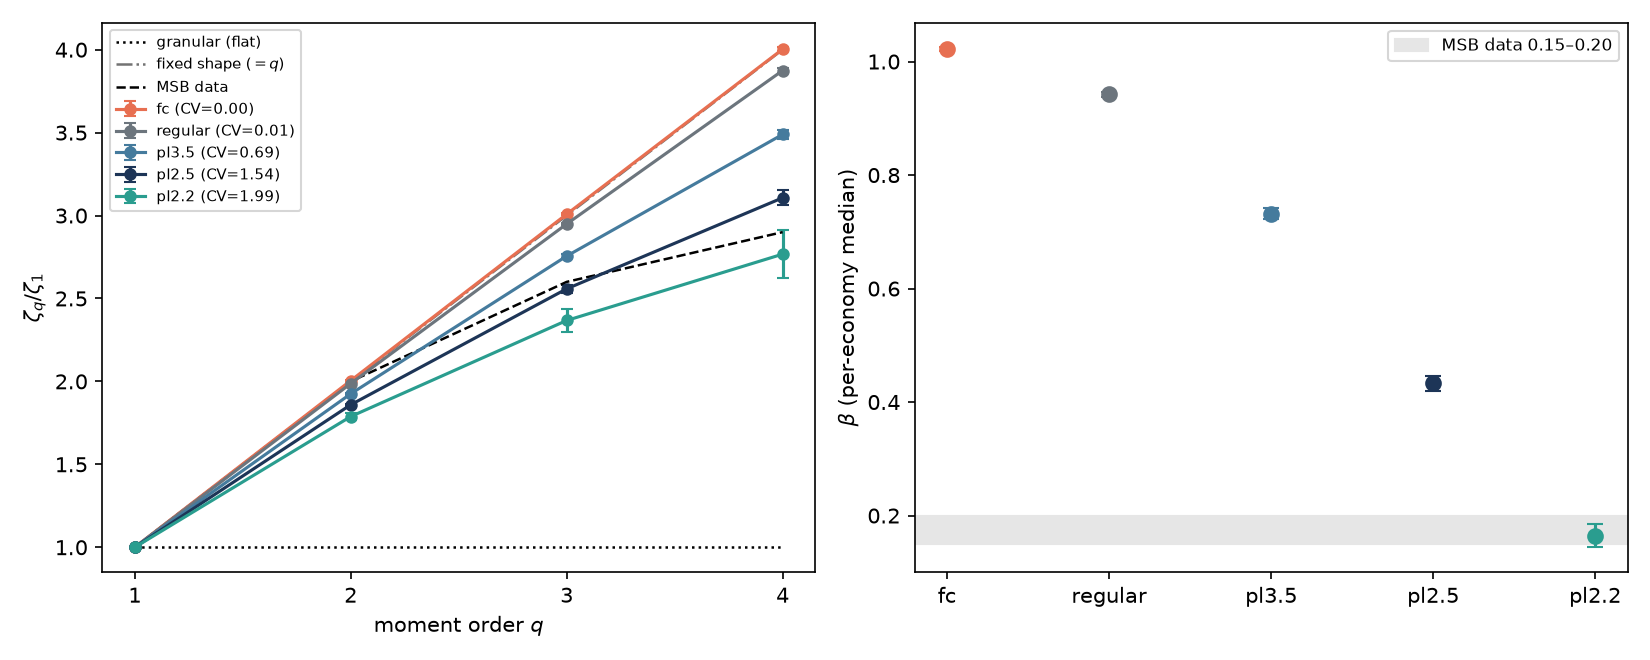
\includegraphics[height=0.52\textheight]{meandeg_topology.png}
  \end{center}
  \begin{itemize}
    \item fully connected and regular graphs: \emph{no} multiscaling
      ($\zeta_q/\zeta_1 \approx 1,2,3,4$) and $\beta \approx 1$,
    \item the degree-tail exponent is the dial: it bends the ratio curve and moves $\beta$,
    \item tail $2.5$: ratios on the data, $\beta = 0.45$; tail $2.2$:
      $\beta = 0.21 \pm 0.07$ inside the empirical band, ratios a few percent low
      --- the graph \alert{brackets} the empirical exponents.
  \end{itemize}
\end{frame}

\begin{frame}{From degree to size: survival under competition}
  \begin{columns}
    \column{0.55\textwidth}
      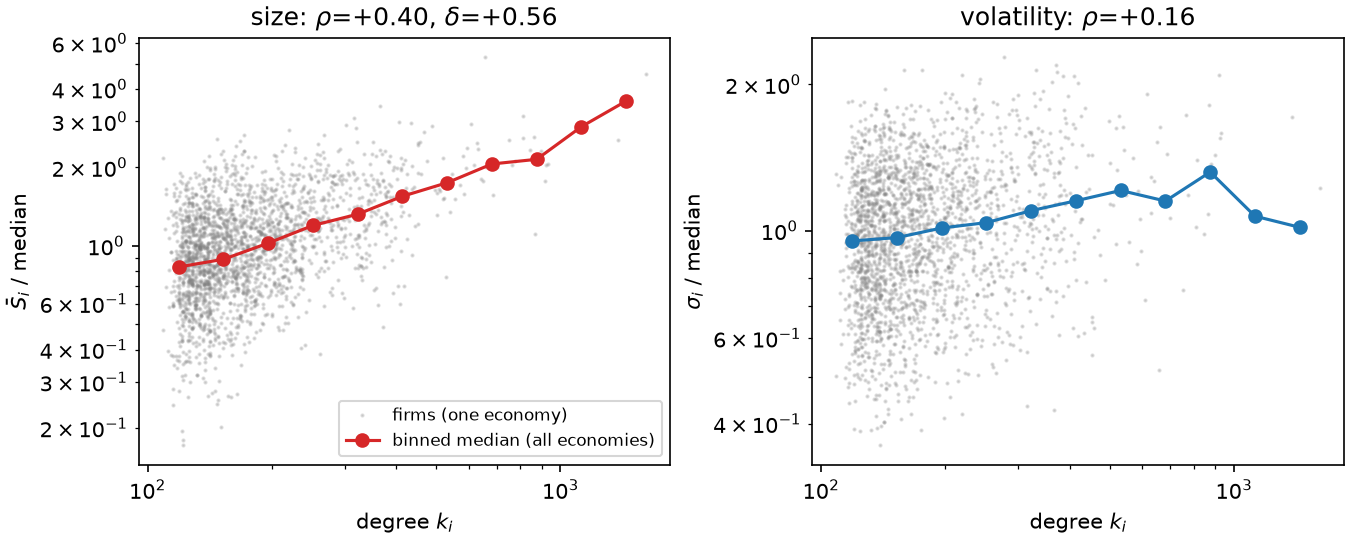
\includegraphics[width=\textwidth]{meandeg_degree_size.png}
    \column{0.42\textwidth}
      How does topology reach a \emph{size}-conditioned law?
      \begin{itemize}
        \item degree sets size: $\bar S \sim k^{\delta}$,
          $\delta = 0.56 \pm 0.02$,
        \item but survival falls with degree ($0.22 \to 0.02$):
          hubs feel coherent competitive pressure $\propto k$,
        \item a balance-of-terms survival criterion, one constant calibrated
          to the aggregate rate, reproduces both curves.
      \end{itemize}
  \end{columns}
\end{frame}

% ---------------------------------------------------------------- 2 min
\begin{frame}{Conclusion}
  \begin{itemize}
    \item A scale-invariant disordered Lotka--Volterra economy on a scale-free graph
      reproduces, \alert{as stationary properties of the interactions},
      the statistics whose failure ruled out the granular picture:
      the size--variance law, the fat tails, and the anomalous multiscaling.
    \item The degree tail of the graph sets the exponents and brackets the empirical
      $\beta \approx 0.15$--$0.20$.
    \item The mechanism is quenched: a firm's role --- size, volatility --- is written
      in the frozen couplings, which is why mean-field order parameters miss it.
  \end{itemize}
  \medskip
  \textbf{Limits}: $\beta$ still drifts with $N$ at accessible sizes (only the moment
  \emph{ratios} converge); exponents are measured, not derived.
\end{frame}

\begin{frame}[standout]
  Thank you
\end{frame}

% ---------------------------------------------------------------- backup
\appendix

\begin{frame}{Backup: a growing, fluctuating economy}
  \begin{center}
    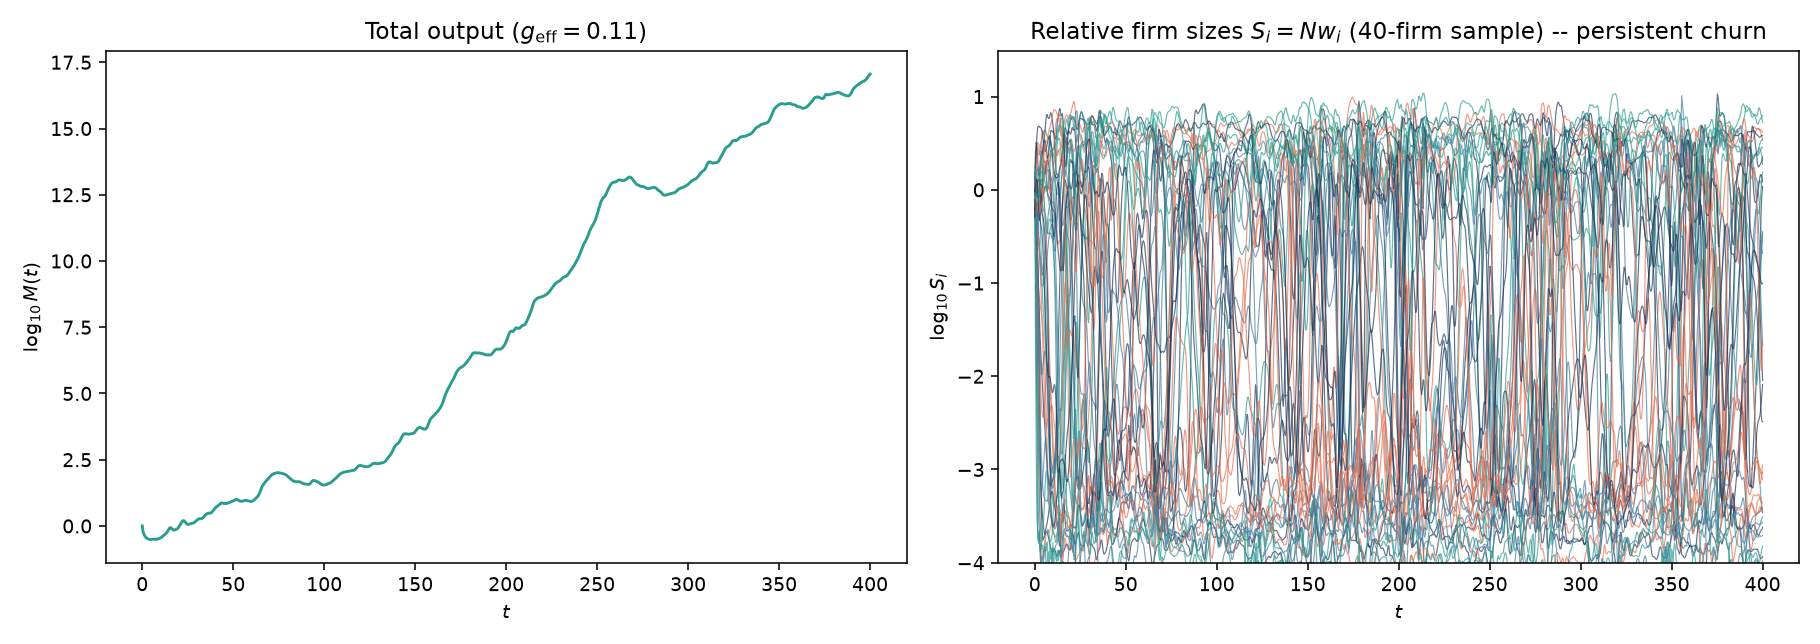
\includegraphics[height=0.58\textheight]{growing_growth_churn.png}
  \end{center}
  \begin{itemize}
    \item $\log m$ climbs at a steady slope over unbounded time --- exponential growth,
      no finite-time singularity (the failure of the absolute model),
    \item relative sizes never settle: persistent chaotic churn of the composition.
  \end{itemize}
\end{frame}

\begin{frame}{Backup: the other two size-conditioned tests}
  \begin{center}
    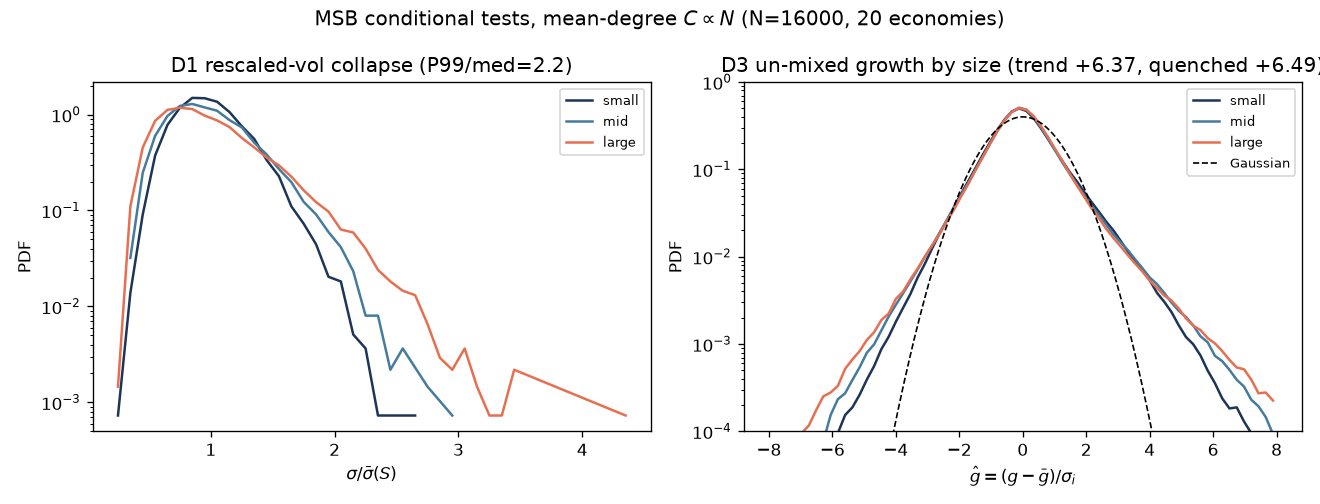
\includegraphics[height=0.58\textheight]{meandeg_conditional.png}
  \end{center}
  \begin{itemize}
    \item per-firm volatility distribution: rescaled shape with a bounded tail,
    \item size-unmixed growth $(g - \bar g)/\sigma_i$: heavy tails that strengthen with size,
  \end{itemize}
  both as in the empirical data.
\end{frame}

\begin{frame}{Backup: finite size}
  \begin{columns}
    \column{0.55\textwidth}
      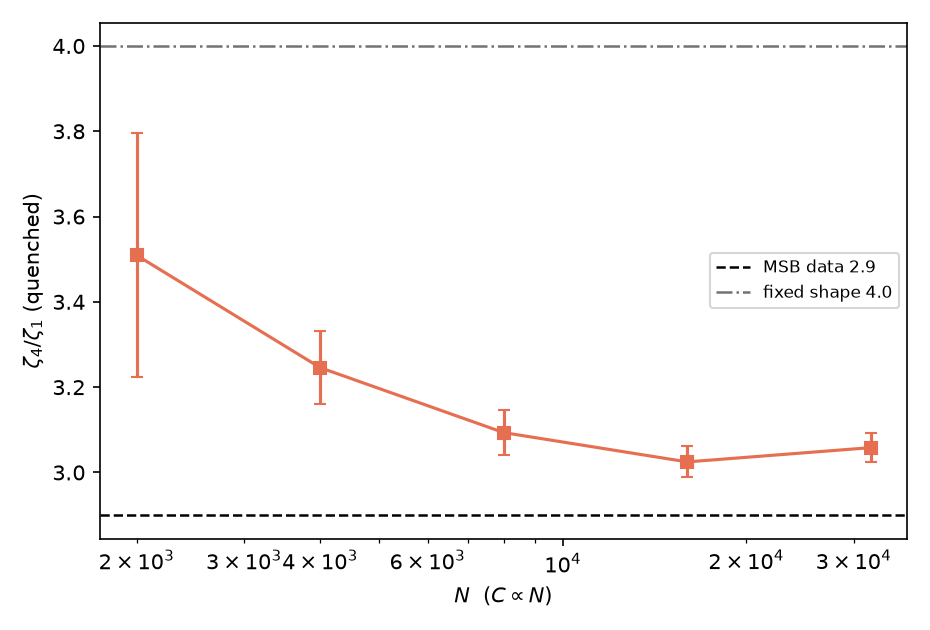
\includegraphics[width=\textwidth]{meandeg_ratio4_vs_N.png}
    \column{0.42\textwidth}
      \begin{itemize}
        \item moment ratios $\zeta_q/\zeta_1$ converge with $N$,
        \item $\beta$ itself still climbs ($0.42 \to 0.49$ over $N = 8000 \to 32000$
          at tail $2.5$) --- no plateau at accessible sizes,
        \item $C \propto N$ (here $N/40$) is required: at fixed $C$ the hub
          over-coupling grows unboundedly and the size--variance law washes out.
      \end{itemize}
  \end{columns}
\end{frame}

\begin{frame}{Backup: the control that kills the effect}
  Normalizing each coupling by the firm's \emph{own} degree,
  $\alpha_{ij} = \mu/k_i + (\sigma/\sqrt{k_i})\,z_{ij}$, equalizes the disorder-field
  variance across firms.
  \begin{itemize}
    \item the graph then cancels out of every size-conditioned statistic:
      no multiscaling, no degree--size structure,
    \item under the standard normalization $\mathrm{Var}\,h_i \propto k_i/C$:
      hubs live in louder environments --- the degree distribution is printed onto
      the firm-level noise,
    \item degree heterogeneity is not incidental; it \emph{is} the mechanism.
  \end{itemize}
\end{frame}

\end{document}
